%!TEX encoding = UTF-8 Unicode
\section{内容3}
\subsection{内容3-1}

\begin{figure}[b]
    \centering
    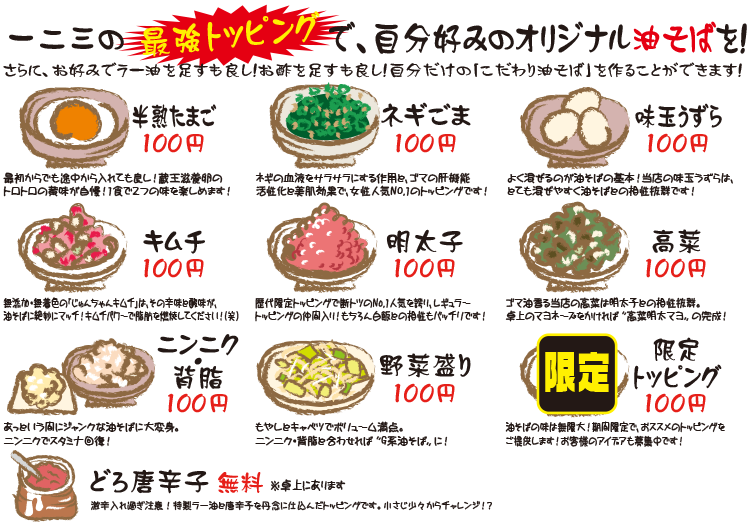
\includegraphics[width=0.85\textwidth]{./fig/hifumi_topping.png}
    \caption{油そば一二三のトッピング}
    \label{LABEL_FIGURE}
\end{figure}

\begin{table}[b]
    \centering
    \caption{表のタイトル}
    \begin{tabular}{|c|c|c|} \hline
        要素1 & 要素2 & 要素3 \\ \hline
        要素4 & 要素5 & 要素6 \\ \hline
    \end{tabular}
    \label{LABEL_TABLE}
\end{table}

参考文献の参照の仕方\cite{meinronbun}によると

\begin{lstlisting}[caption=Hello World,label=dockerfile]
#include<stdio.h>
int main(){
    printf("Hello world!");
}
\end{lstlisting}
